%%
%% LaTeX template for SC18 Scientific Visualization & Data Analytics
%% Showcase submissions.
%%
%% SciVis Showcase submissions must be formatted using Elsevier's document
%% class `elsearticle'. The necessary class and bibliography style files
%% are included, but the original package is posted on CTAN at
%%
%%     https://ctan.org/tex-archive/macros/latex/contrib/elsarticle
%%

%% SC SciVis Showcase submissions should use the elsarticle document class
%% with options `final,5p,times,twocolumn`.
\documentclass[final,5p,times,twocolumn]{elsarticle}
\hyphenation{ParaView}
%% The amssymb package provides various useful mathematical symbols
\usepackage{amssymb}
%% The amsthm package provides extended theorem environments
%% \usepackage{amsthm}

%% Command used to change the verbatim environment font. This is
%% used for the template's instructions and does not need to remain
%% for papers using this template.
\makeatletter
\newcommand{\verbatimfont}[1]{\def\verbatim@font{#1}}%
\makeatother

\usepackage{url}
\usepackage{bm}

%% Accepted SC SciVis Showcase submissions will be published in
%% Parallel Computing.
\journal{Parallel Computing}

\begin{document}

\begin{frontmatter}

%% Title, authors and addresses

%% use the tnoteref command within \title for footnotes;
%% use the tnotetext command for theassociated footnote;
%% use the fnref command within \author or \address for footnotes;
%% use the fntext command for theassociated footnote;
%% use the corref command within \author for corresponding author footnotes;
%% use the cortext command for theassociated footnote;
%% use the ead command for the email address,
%% and the form \ead[url] for the home page:
%% \title{Title\tnoteref{label1}}
%% \tnotetext[label1]{}
%% \author{Name\corref{cor1}\fnref{label2}}
%% \ead{email address}
%% \ead[url]{home page}
%% \fntext[label2]{}
%% \cortext[cor1]{}
%% \address{Address\fnref{label3}}
%% \fntext[label3]{}

\title{Volume Renderings of Sheared Thermal Convection}

%% use optional labels to link authors explicitly to addresses:
%% \author[label1,label2]{}
%% \address[label1]{}
%% \address[label2]{}

\author[CSCS]{Jean M. Favre}
\author[Twente]{Alexander Blass}

\address[CSCS]{Swiss National Supercomputing Center (CSCS), Via Trevano 131, CH-6900 Lugano, Switzerland}
\address[Twente]{Physics of Fluids Group, Max Planck Center for Complex Fluid Dynamics,
J. M. Burgers Center for Fluid Dynamics and MESA+ Research Institute,
Department of Science and Technology,
University of Twente, P.O. Box 217, 7500 AE Enschede, The Netherlands}

\begin{abstract}

We present visualizations of sheared thermal convection in large scale
wall-bounded turbulent flow simulations. The visualizations are based on volume
renderings of the temperature field. To address the needs of supercomputer users
with different hardware and software resources, we evaluate different implementations
supported in the ParaView \cite{Ahrens2005} environment: two GPU-based solutions
with Kitware's native volume mapper or NVIDIA's IndeX library, and a software-only
OSPRay-based implementation.

\end{abstract}

\begin{keyword}

%% keywords here, in the form: keyword \sep keyword
Scientific Visualization \sep High Performance Computing \sep Naviers-Stokes Solver \sep Direct Numerical Simulation \sep Computational Fluid Dynamics

\end{keyword}

\end{frontmatter}

%% \linenumbers

\begin{figure}[!hbt]
	\centering
	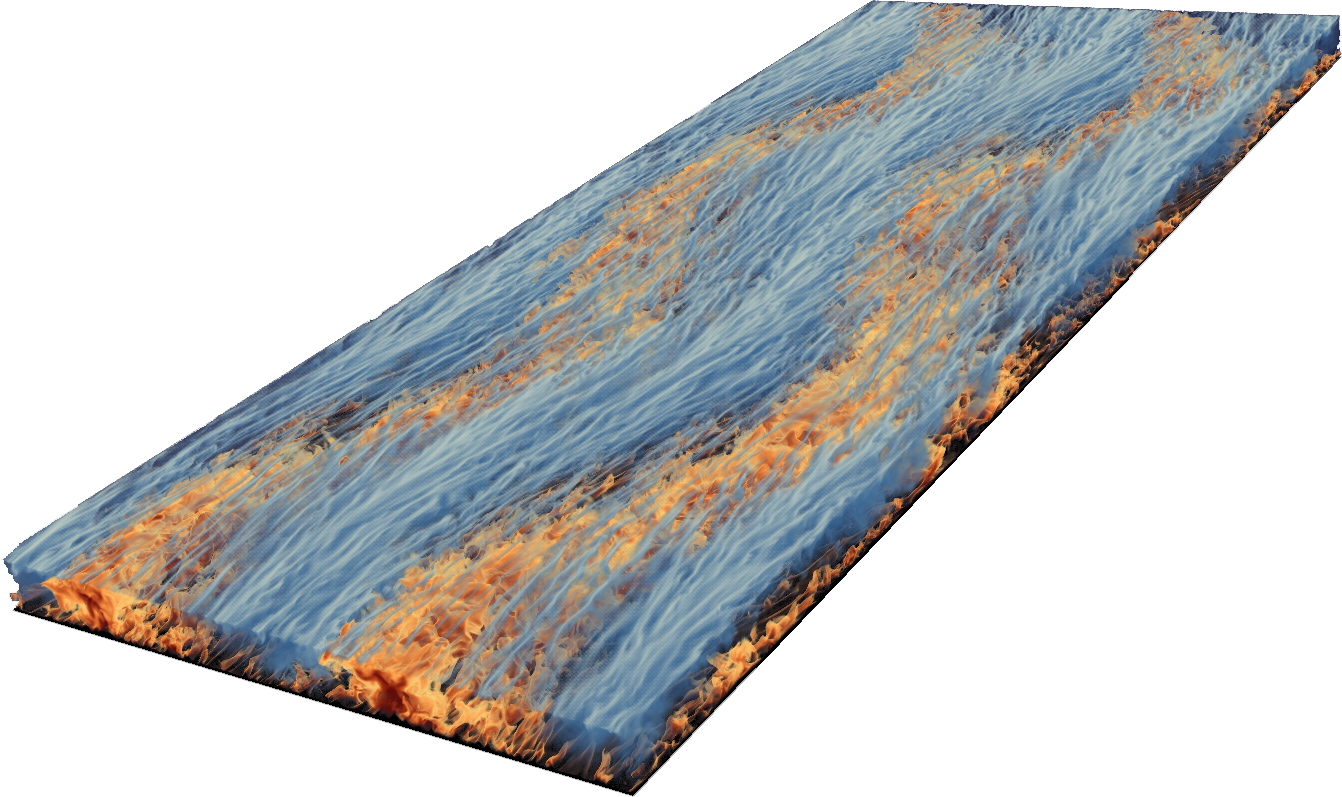
\includegraphics[width=\linewidth]{flowfield}% 
	\caption{\label{fig:flowfield} Instantaneous snapshot of the three-dimensional temperature field of sheared thermal convection at $ Ra=4.6 \times 10^6 $ and $ Re=6000 $ \cite{bla18}.}
\end{figure}

%% main text
\section{Introduction}
\label{sec:Introduction}

Oceans play a big role in the nature of our planet. About $ 70 \% $ of our earth
is covered by water. Strong currents are transporting warm water around the world
and therefore don't only make life possible, but also allow us to harvest its
power producing energy. But humanity tends to easily forget that oceans also
yield a much more deadly side. Floods and tsunamis can easily annihilate whole
cities and destroy life in seconds. The earth's climate system is also very much
linked to the circulation in the ocean due to its large coverage of the earth's surface.
One has to treat the ocean with respect and carefulness, but it is unambiguously
clear that humanity and its science is just attempting to reach the first step on
an oceanic staircase to understanding nature.

\section{Numerical Simulations}

A more fundamental setup of this natural mechanism is sheared thermal convection.
Many processes in nature can be based on heat and momentum
transfer and therefore interaction between buoyancy \cite{ahl09} and shear \cite{smi11,bar07}. Direct
numerical simulations (DNS) were performed with the second-order finite-difference
code \textit{AFiD} \cite{poe15c} in which the three-dimensional non-dimensional
Navier-Stokes equations with the Boussinesq approximation on a staggered grid are solved:

\begin{equation} %NS equation
\frac{\partial \boldsymbol{u}}{\partial t} + \boldsymbol{u} \bm{\cdot} \bm{\nabla} \boldsymbol{u} =-\bm{\nabla} P + \left(\frac{Pr}{Ra} \right)^{1/2} \nabla^2\boldsymbol{u}+\theta \hat{z}, 
\label{eqn:NS}
\end{equation}

\begin{equation} %NS equation
\bm{\nabla} \bm{\cdot} \boldsymbol{u} =0,
\label{eqn:div}
\end{equation}

\begin{equation} %Temp equation
\frac{\partial \theta}{\partial t} + \boldsymbol{u} \bm{\cdot} \bm{\nabla} \theta = \frac{1}{(Pr Ra)^{1/2}} \nabla ^2 \theta.
\label{eqn:temp} \\[8pt]
\end{equation}

We use $ \boldsymbol{u}=u(\boldsymbol{x},t) $ as the velocity vector with streamwise, spanwise and wallnormal components. $ \theta $ is the non-dimensional temperature ranging from $ 0 \leq \theta \leq 1 $. The simulations are performed in a computational box with periodic boundary conditions in streamwise and spanwise directions and confined by a heated plate below and a cooled plate on top. The shearing of the flow is implemented by a Couette flow setting where both top and bottom plates of the flow are moved in opposite directions with the speed $ u_w $ keeping the average bulk velocity at zero and therefore minimizing dissipation errors. The domain size is ($ L_x \times L_y \times L_z $) = ($ 9\pi h \times 4\pi h \times h $) using a grid of ($ n_x \times n_y \times n_z $) = ($ 6912 \times 3456 \times 384 $) which is homogeneously distributed in the streamwise and spanwise directions and clustered with an error-function $ \eta(\xi)=erf(2\xi)/erf(2) $ in wallnormal direction.

The open sourced finite-difference Navier-Stokes solver \textit{AFiD} \cite{poe15c} was written in Fortran 90 to study large-scale wall bounded turbulent flow simulations. In collaboration with NVIDIA, USA, the code was ported in its newest version to a GPU setting using a MPI and CUDA Fortran hybrid implementation optimized to run and solve large flow fields \cite{zhu18b}.

For this visualization showcase, data from Blass et al. \cite{bla18} was used, where a parameter study over different input parameters was conducted to study the influence of such to the flow field. Control parameters were the temperature difference between the top and bottom plates as the strength of the thermal forcing, non-dimensionalized as the Rayleigh number (Eqn. \ref{eqn:Ra}), and the wall velocity as the strength of the shear forcing, non-dimensionalized as the wall shear Reynolds number (Eqn. \ref{eqn:Re}), while keeping the Prandtl number (Eqn. \ref{eqn:Pr}), which is the ratio of thermal and viscous viscosity of a fluid, at unity. The equations read:

\begin{equation} %Ra
Ra= \frac{\beta gh^3\Delta T}{\kappa\nu}, 
\label{eqn:Ra} \\[8pt]
\end{equation}

\begin{equation} %Re_w
Re_w= \frac{hu_w}{\nu},
\label{eqn:Re} \\[8pt]
\end{equation}

\begin{equation} %Pr
Pr= \frac{\nu}{\kappa},
\label{eqn:Pr} \\[8pt]
\end{equation}


where $ \beta $ is the thermal expansion coefficient of the fluid, $ g $ the
gravitational acceleration, $ \kappa $ the thermal diffusivity, $ \nu $ the
kinematic viscosity of the fluid, $ h $ the distance between the plates and
$ u_w $ the wall velocity.

\begin{figure}
	\centering
	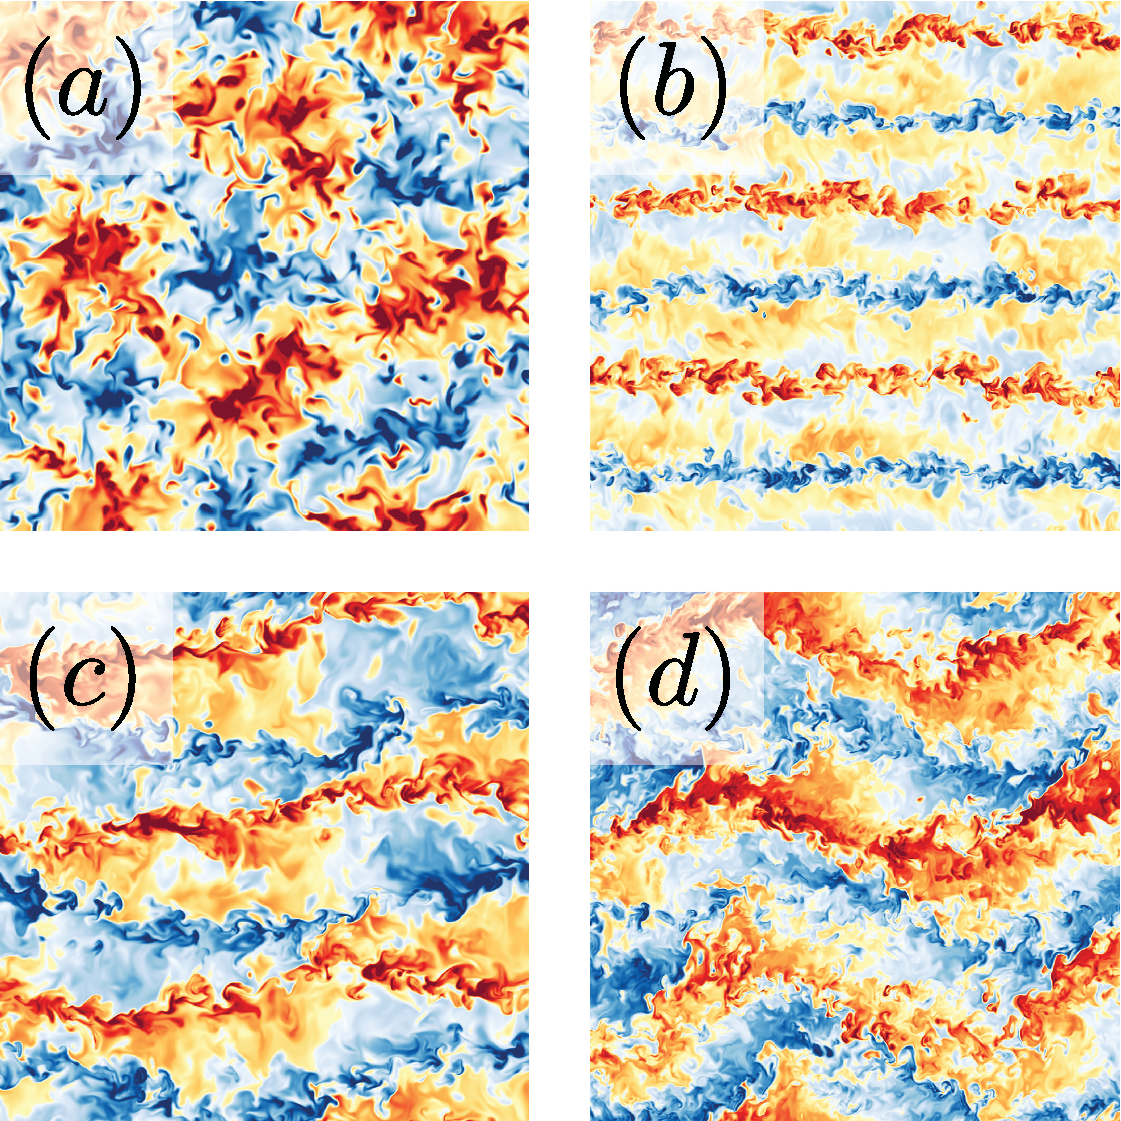
\includegraphics[width=\linewidth]{squaredoverview}% 
	\caption{\label{fig:overview} Zoomed instantaneous snapshots of temperature fields
of a sheared and thermally forced flow transitioning through all flow regimes
for $ Ra=2.2 \times 10^6 $ and (a) $ Re=0 $, (b) $ Re=2000 $, (c) $ Re=3000 $, (d) $ Re=6000 $.}
\end{figure}

In Fig. \ref{fig:overview} we present instantaneous snapshots of temperature
fields at mid height in different flow regimes. It can be observed that the flow passes from a
thermally dominated regime with large plumes (Fig. \ref{fig:overview}a) into a
regime where the mechanical forcing is dominant. Here, large-scale meandering
structures can be observed (Fig. \ref{fig:overview}d). To transition between the
regimes, the flow has to pass a transitional stage, in which the thermal plumes
get stretched into large streaks (Fig. \ref{fig:overview}b). If the shearing is
further increased, these streaks become instable and start meandering into the
final flow state (Fig. \ref{fig:overview}c).

In turbulent flows it is very important to research how certain characteristic
parameters are influenced by the flow. Changing flow structures might have a
supporting effect or may disrupt a previously transport-favorable flow situation. 
In thermal convection, such parameter is the heat transfer, non-dimensionally
defined through the Nusselt number:

\begin{equation} %Nusselt equation
Nu= \frac{Qh}{\kappa \Delta \theta}
\label{eqn:nusselt} \\[8pt]
\end{equation} 

While two-dimensional visualizations are very helpful in understanding the behavior of the large-scale structures, they don't show the complete scientific picture. They give a good indication of the flow behavior, but to understand thermal turbulence, it is vital to see the whole flow field and dynamic interaction of turbulent structures with each other.

To have the chance to observe the flow while evolving and transitioning through different regimes is a great chance not only to statically observe different flow states at fixed locations in space, but to actually follow the flow on its path to develop thermal plumes, streaks and meandering structures.

\begin{figure}
	\centering
	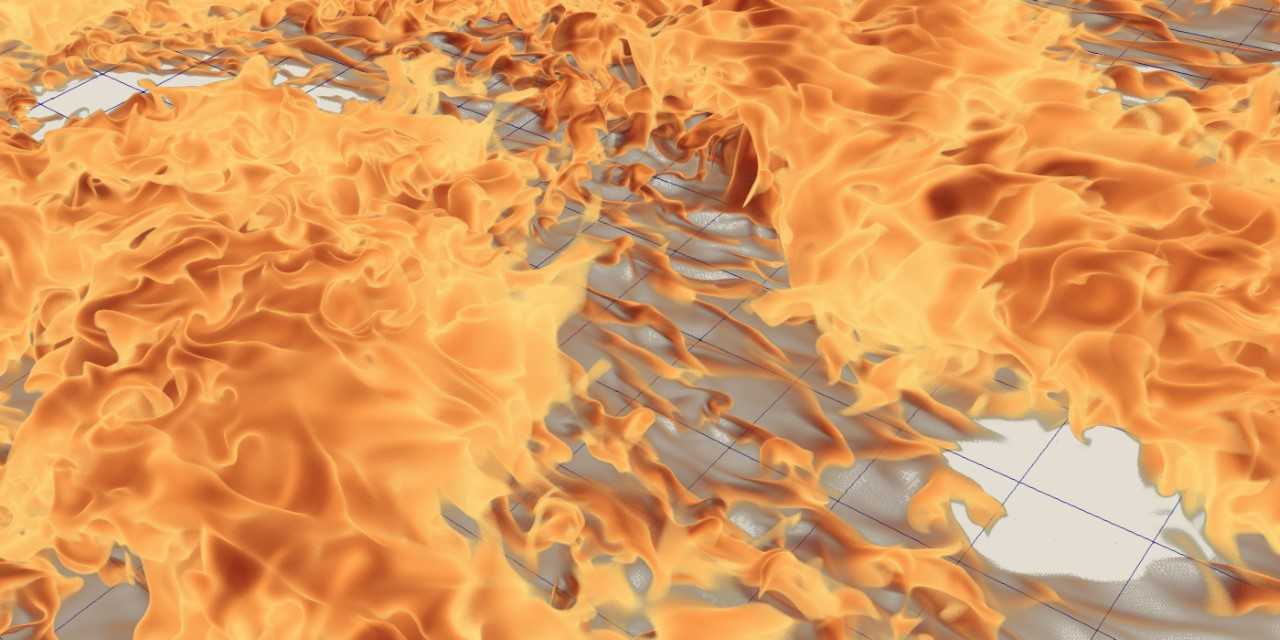
\includegraphics[width=\linewidth]{smallscale}% 
	\caption{\label{fig:smallscale} Zoom of an instantaneous snapshot of the temperature field at $ Ra=2.2 \times 10^6 $ and $ Re=6000 $.}
\end{figure}

It has been previously shown in thermal convection that the large thermal plumes can be traced until very close to the heated and cooled plates \cite{ste18}. So it is very important to also observe the emergence of structures close to the boundary layer. The detailed visualizations presented in this paper allow us to not only follow the large-scale structures, but also the interaction of small-scale structures much closer to the plates (Fig. \ref{fig:smallscale}).\\

The mesh used in our simulations is made of $ 6912 \times 3456 \times 384 $ grid points.
The temperature scalar field stored as \it{float32} \rm takes 36 Gb of memory, an
overwhelming size to handle on a normal desktop. Using different parallel programming
paradigms has enabled us to provide an engaging environment
to promote interactive tuning of visualization options and high productivity for movie
generation. We use ParaView v5.5.2, a world-class, open-source, multi-platform data analysis and
visualization application installed on Piz Daint. Piz Daint, a hybrid Cray XC40/XC50 system,
is the flagship supercomputer of the Swiss National HPC service. We have deployed
and tested several solutions within ParaView where parallelism is expressed
at different degrees: data-parallel visualization pipelines with GPU-based renderings,
or multi-threaded parallelism for software renderings.

\section{Volume rendering libraries and setup}

Visualization of 3D scalar fields is a very mature field. Many techniques are
available to get some sense of the 3D nature of the data, and its variations
through the volume. Surface-based renderings with isosurface thresholds or
slicing planes have a great appeal in that they are easy to use, but volumetric
renderings, first made popular in medical applications, are also a great fit for
scalar visualizations, especially in the realm of time-dependent outputs.
\newline
ParaView's "Smart" VolumeMapper is an image mapper
that will delegate to a specific volume mapper based on rendering parameters and
available hardware. It is a convenient
wrapper to test multiple options.
\newline
The largest partition of the Piz Daint supercomputer
nodes is equipped with one Intel Xeon E5-2690 (12 cores, 64 Gb RAM) and one NVIDIA
Tesla P100 GPU (16 Gb RAM), so our priority is to evaluate the GPU-based implementations.
ParaView's "Ray Cast Only" mode is also available but we have found its performance far
below the other options, and we discarded its use. We aim to test ParaView's GPU
ray casting implementation, against an NVIDIA-developed custom library called
IndeX, and against a CPU-only solution, to give a valid option to users of
supercomputers not equipped with GPUs.
Our performance evaluation is based on ParaView's benchmarking Python source
code\footnote{source code found in ./Wrapping/Python/paraview/benchmark/}.
\newline
For all methods used, we have ignored disk-based I/O costs. There is often quite
a bit of variability when running on a large distributed file system shared by
hundreds of users. Our motivations are rendering-centered, and two-fold:
evaluate the memory cost and resources (CPU, GPU) required to get a first image
on the screen, and see if color/opacity transfer
function editing, as well as other image tuning can be done in real time, using
any of the three methods proposed. In the evaluation of performance costs, ParaView's
benchmark code enables fully automatized testing with a careful management of
double buffering, saving images from the back buffer to bypass driver optimizations.

In the two GPU-based methods evaluated, we use an EGL-based rendering layer,
relaxing the need to have a server-side X-Windows server running on the compute node.
This enables headless, offscreen rendering with GPU acceleration. We note however that although
the GPUs provide phenomenal compute power, they are limited by the available memory
(16 Gb on our NVIDIA's Pascal GPUs). For the full size of our simulations outputs, we are actually forced to use data-parallel
pipelines on multiple nodes to use the aggregate memory of the different GPUs.
\newline
Our third option, however, uses OSPRay and software rendering and does not suffer
from a memory hard limit. Compute nodes are easily and often found with large memory
banks. We use Piz Daint's high memory nodes with 128 Gb of RAM, where our mesh of
over 9 billion voxels can be rendered easily on a single node.

\begin{figure}
	\centering
	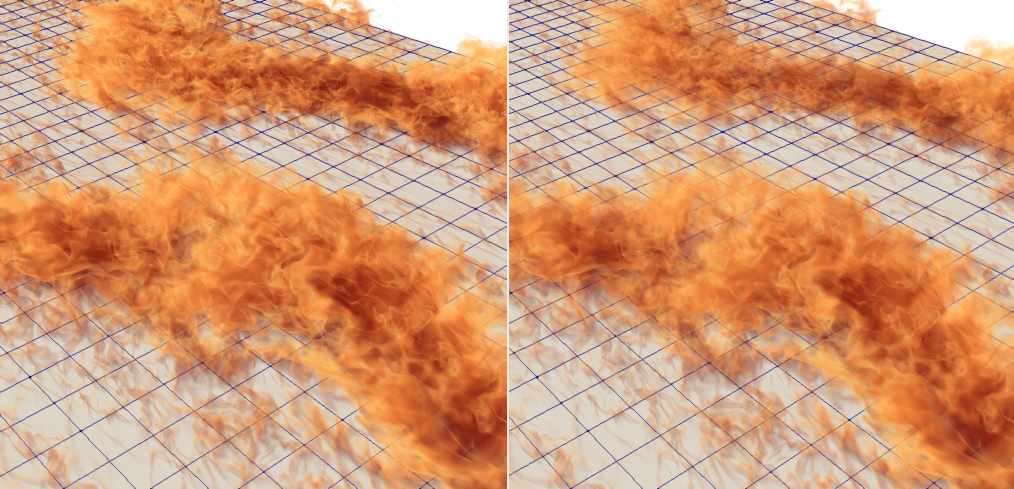
\includegraphics[width=\linewidth]{fig2}% 
	\caption{\label{fig:gpucloseup} Volume renderings of temperature with ParaView's
Smart Shader (left), and with NVIDIA IndeX (right)}
\end{figure}

\subsection{ParaView's GPU Ray Casting} \label{smart}

ParaView's most efficient mapper - if the GPU hardware supports it - is a volume
mapper that performs ray casting on the GPU using fragment programs. Care must
be taken when evaluating and comparing the different approaches. We highlight the
fact that in this preferred mode, ParaView converts the 32-bit float data to 16-bit
integer. In Fig. \ref{fig:gpucloseup} (left), we note very small differences of illumination with the
NVIDIA IndeX-rendered image at full 32-bit resolution,
but no degradation due to down-converted data.

\subsection{NVIDIA IndeX} \label{index}

NVIDIA IndeX \cite{NVIDIAIndeX} is a commercial 3D volumetric visualization SDK developed to enable
the visualization of massive datasets. NVIDIA has worked in tandem with Kitware to
bring an implementation of IndeX to ParaView, and we have enjoyed the benefits
of a close partnership between the Swiss National Supercomputing Center (CSCS),
and NVIDIA, to be able to use IndeX in a multi-GPU setting. We use the ParaView
plugin v2.1 with the core library NVIDIA IndeX 1.5 (build 299900.2384). In
Fig. \ref{fig:gpucloseup} (right), an NVIDIA IndeX rendering is done with identical
color and opacity transfer functions as used in \ref{smart}.
Small differences can be accounted for with a non uniform interpretation of the sampling rates
for the scalar opacity unit distance as coded in the three proposed implementations.

\subsection{Intel OSPRay}

OSPRay \cite{OSPRay} is a ray tracing framework for CPU-based rendering. It supports advanced 
shading effects, large models and non-polygonal primitives. OSPRay can distributes 
"bricks" of data as well as "tiles" of the framebuffer, although in our current
implementation, we only use brick subdivisions. The Texas Advanced Computing Center
has developed a ParaView plugin which enables us to test the possibility of
using a ray-tracing based rendering engine for volumetric rendering. This is
the best solution for clusters where no GPU hardware is available.

In the case of OSPRay, we rely on a different parallel computing paradigm.
The emphasis is no more on data parallelism, but rather on multi-threaded execution.
A complete \it{software-only} \rm ParaView installation was deployed with an LLVM-based and
OpenGL Mesa layer. We used Mesa v17.2.8, compiled with LLVM v5.0.0, and the
OSPRay v1.6.1 library to provide a very efficient multi-threaded execution path
taking advantage of Piz Daint's alternate partition of compute nodes. These nodes
are built with two Intel Broadwell CPUs (2x18 cores and 64/128 Gb RAM). We run
ParaView with SLURM's option "--cpus-per-task=72 --ntasks-per-core=2", effectively
taking full advantage of the multi-threading exposed by the LLVM and OSPRay libraries. 

\subsection{Parallel Image Compositing}

ParaView's default mode of parallel computing is to use data-parallel distribution,
whereby sub-pieces of a data grid are processed through identical visualization
pipelines. To combine the individual framebuffers of each computing nodes,
ParaView uses Sandia National Laboratory's IceT \cite{Moreland2011} compositing
library. We use it in its default mode of operation doing sort-last compositing
for desktop image delivery. We note here that NVIDIA's IndeX uses a proprietary
compositing library, so for the IndeX tests only, we disable ParaView's default
image compositor.

\section{Volume rendering of the thermal convection}

\begin{figure}[!hbt]
	\centering
	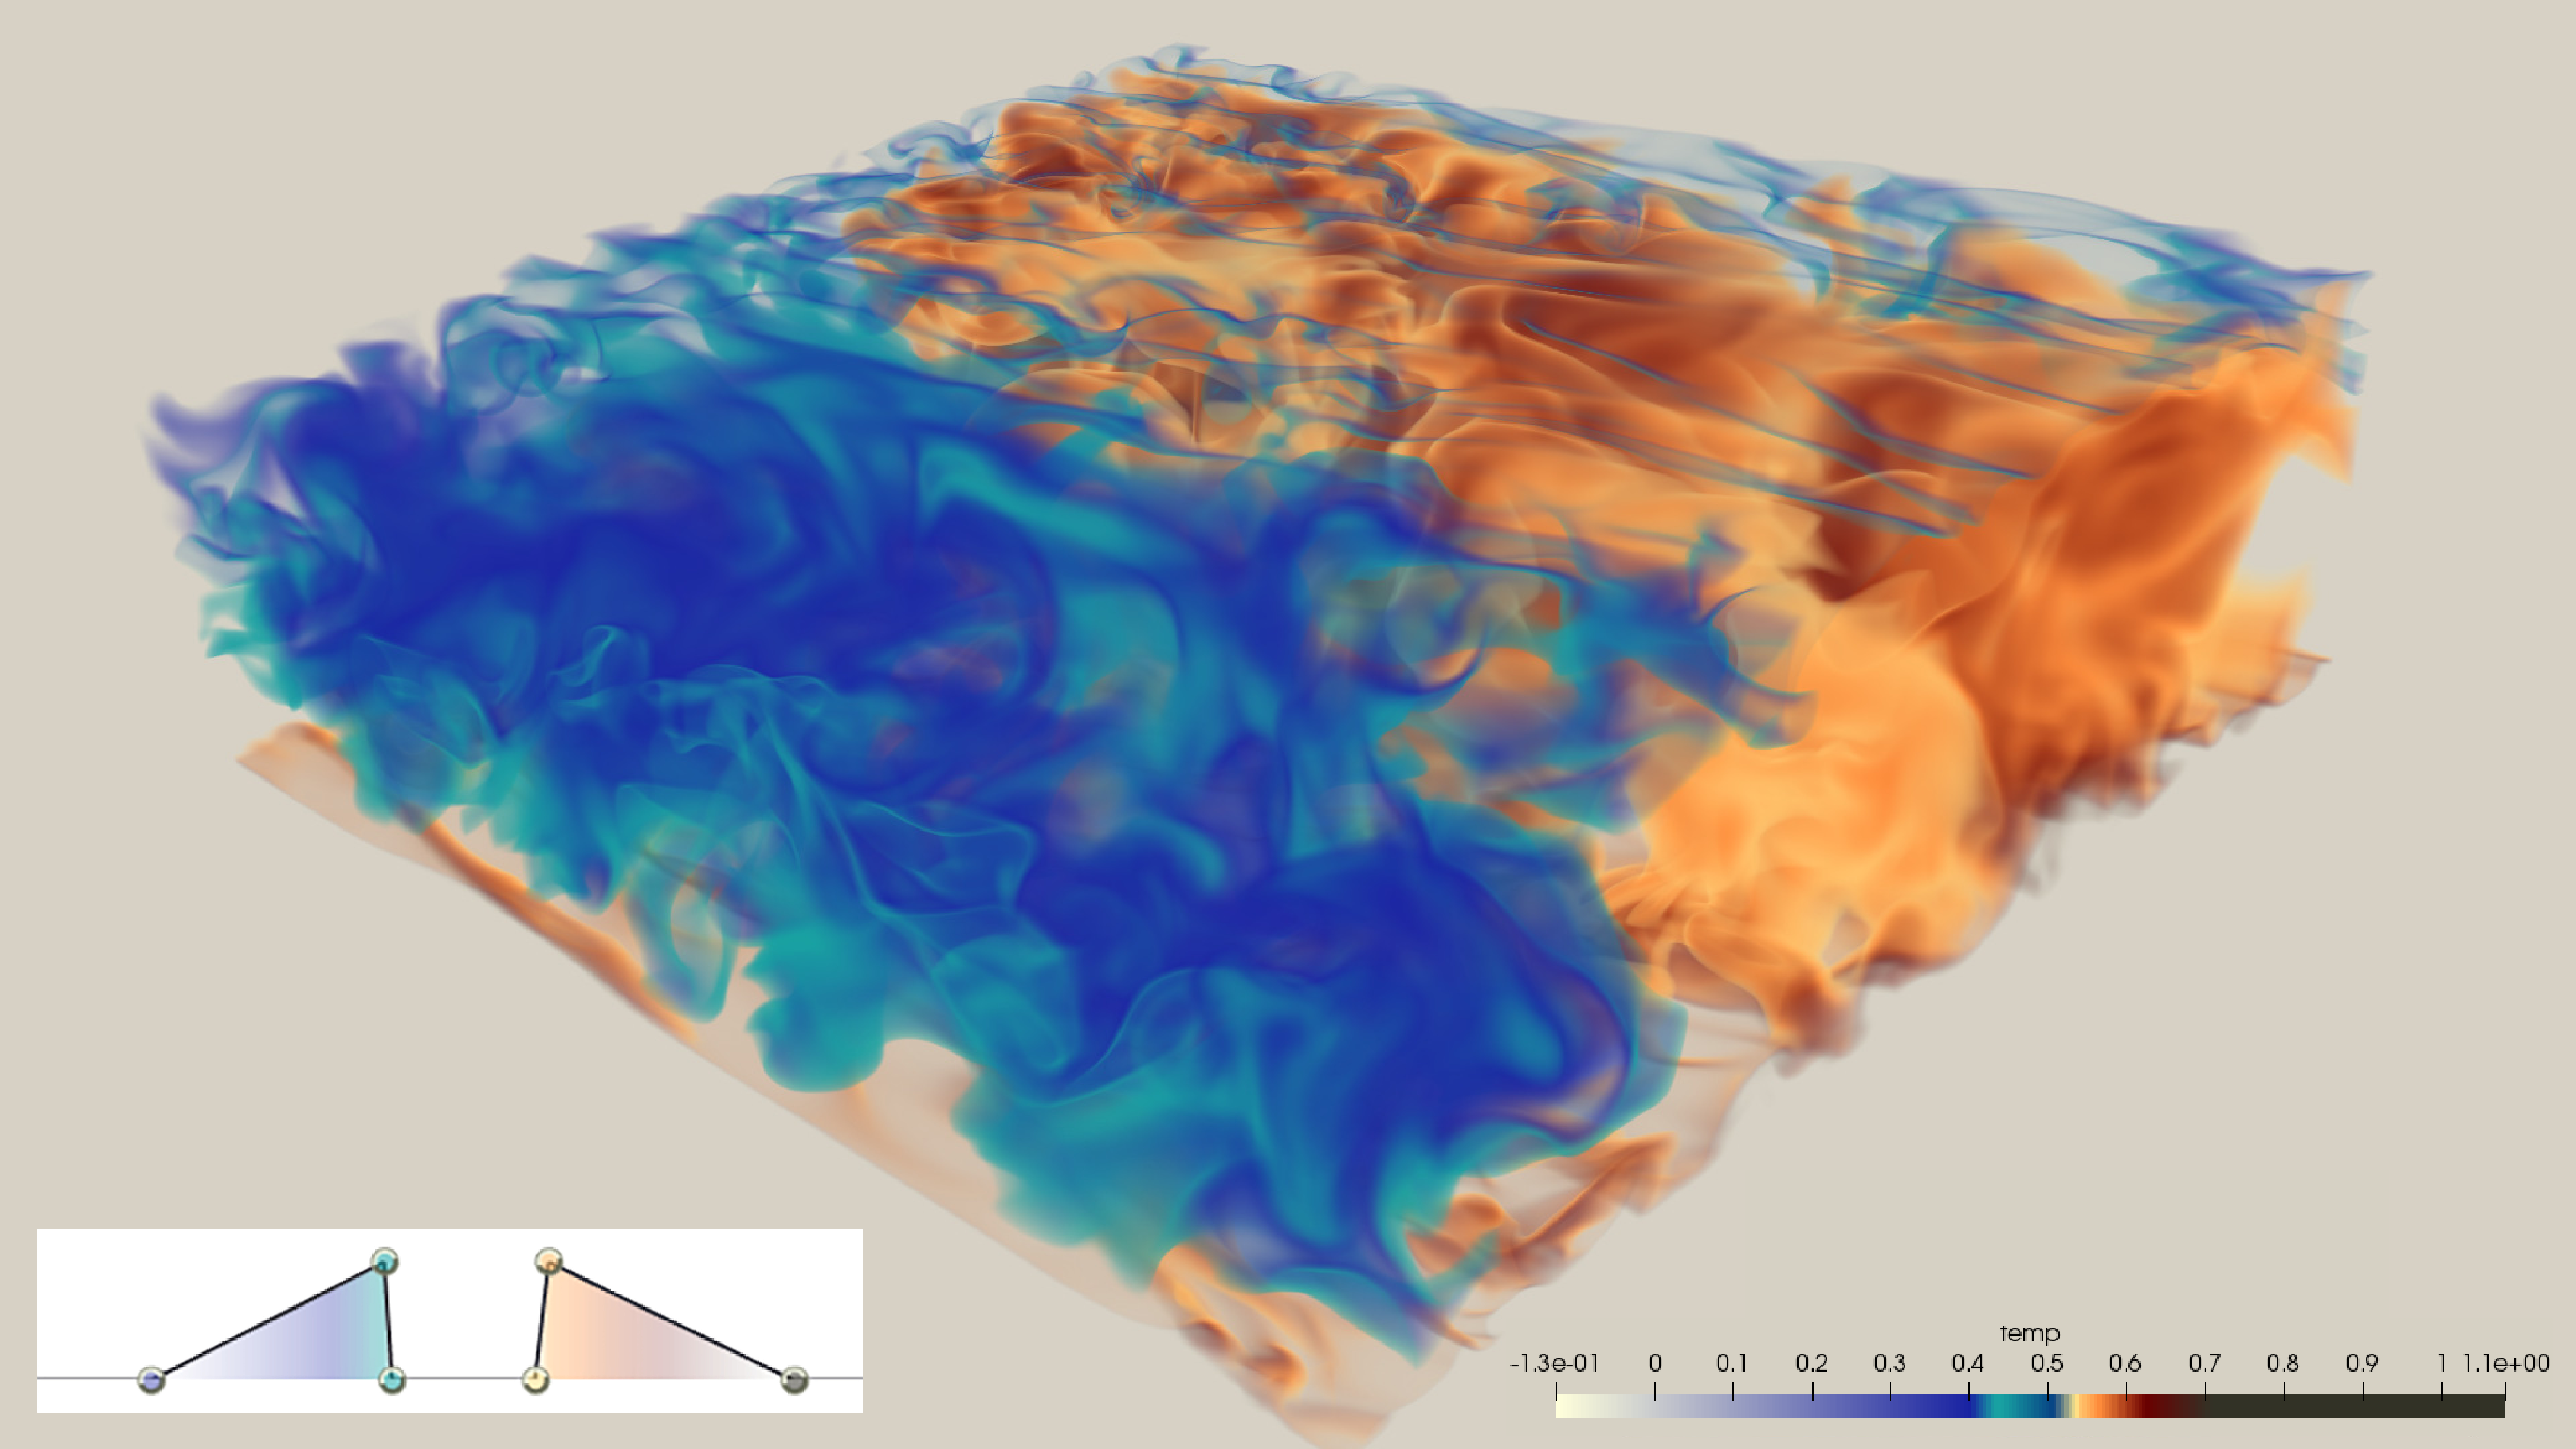
\includegraphics[width=\linewidth]{zoom0000}% 
	\caption{\label{fig:zoom} Example of a color and opacity transfer functions to highlight hot and cold plumes.}
\end{figure}


In visualizing the temperature field, we seek to highlight the turbulence which
is best shown by clearly differentiating between cold and hot regions to see how
they interact with each other, as seen in Fig. \ref{fig:zoom}. Our movie animation shows an initial phase where
region of blue tint is superposed on top of the hotter region. Plumes emerging
from the bottom and mixing into the cold regions highlight this phenomenon.

\subsection{Visual effects}

When presented with multiple visualizations including different illumination and
shading, the scientists actually preferred the renderings which emphasize the
amorphous nature of the field data. As can be seen in Fig. \ref{fig:shadings},
shading based on gradient estimation offers little improvement because our data
does not have strong gradients, and the use of shadows which at first might seem
more appealing, produces images with a strong \it{surface-like} \rm look, which
we discarded upon further analysis.

\begin{figure}
	\centering
	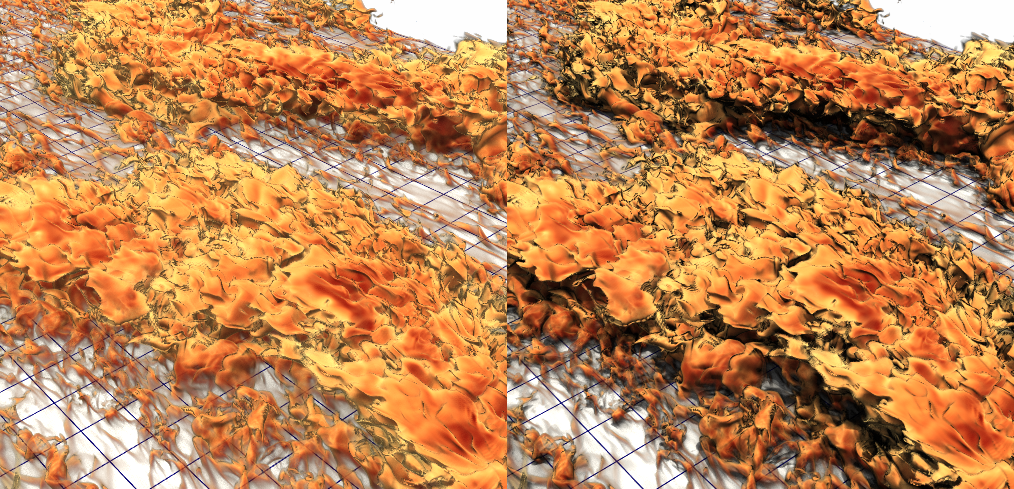
\includegraphics[width=\linewidth]{fig2montage}% 
	\caption{\label{fig:shadings} Volume rendering with shading based on gradient
estimation (left), and with OSPRay-enabled shadows (right)}
\end{figure}


\subsection{Rendering costs on a single node}

Volumetric rendering at this scale of grid has a non significant cost which we
briefly document here. Creating the first frame after data has been read in memory,
 i.e. the startup cost has a great impact in having users adopt a particular implementation.
In a \it{post-hoc} \rm visualization, data would be read from disk; in an \it{in-situ} \rm
scenario, data might have to be converted to VTK data structures. Thus, we measure performance
after the time ParaView has collected all the data and created a bounding-box representation. This startup cost for the first image is also of paramount importance in a movie-making scenario, where data are read from disk, a single image is computed, and the whole visualization pipeline and hardware resources are flushed to visualize the next timestep.
\newline
We summarize in Table \ref{tab:firstframe-tab} the time from when volumetric rendering options are enabled, triggering the building of internal structures until the first frame appears.
To be able to measure the memory cost on a single node, we restricted our test sample to a quarter-size domain of the original grid, i.e. 2.28G voxels ($ 1730 \times 3455 \times 384 $).

\begin{table}[htb]
  \centering
  \caption{
    Initialization and memory costs for a quarter-size domain on one node.
  }
  \label{tab:firstframe-tab}

  \begin{tabular}{lccc}
    \hline
    Rendering library & Startup & pvserver task\\
    \hline
    OSPRay & 2.1 secs &  27.6 Gb \\
    ParaView GPU Mapper & 7.7 secs &  25.8 Gb \\
    NVIDIA IndeX & 15.7 secs &  21.1 Gb\\
    \hline

  \end{tabular}
\end{table}

The high initial setup cost incurred with the NVIDIA IndeX library is due to higher volume transfer between CPU and GPU, a cost that increases further when in parallel mode, as the current
implementation of IndeX will trigger re-execution of the data I/O because of larger than usual ghost layer requests. Work is in progress\footnote{personal communication with NVIDIA Dev. team} to minimize this impact in a future version of the plugin.
\newline
If memory costs are substantial, more nodes, and/or more GPUs will be required,
increasing the run-time cost of the visualization. Our data domain is quite large
indeed, and we are not able to load a half-size domain on a single GPU node. Indeed, both
the 64 Gb RAM on the node and the 16 Gb RAM on the GPU are hard limitations. The OSPRay-based software rendering is one way to alleviate this problem. We can load the full size
domain on a single node of  the multi-core partition of Piz Daint with dual-Xeon
chips and 128 Gb of RAM. We measured again the startup cost for the first image
using 72 execution threads and found them to increase linearly with grid dimensions.
We tested the quarter-size, half-size and the full domain and report the delivery
of the first image in 2.1, 4.0, and 8.0 seconds, respectively. The associated cost
in RAM is also linear, at 27.6 Gb, 55.1 Gb and 110 Gb, respectively.
 
After the first frame has been built, our experience is that renderings
are done at interactive speed with all three libraries tested.
Color and opacity transfer functions editing is also interactive and very intuitive.
 We ran scripted navigation scenarios through a static domain loaded in memory
at HD (1920x1080 pixels) and 4K UDH (3840x2160 pixels) resolutions.

\subsection{Rendering the full domain in parallel}

We have discussed the fact that the two GPU-based rendering solutions
are limited by the available GPU memory. A nearly 9G voxels dataset just will
not fit on a single GPU. To enable our visualization, we must use a parallel 
set of nodes. We measure again the initial cost for the first image
(after all I/O has been done), and also the frame rate achieved in a scripted
animation loop. Table \ref{tab:parallelgpu-tab} summarizes our findings. As noted earlier,
the NVIDIA IndeX library sends the full 32-bit resolution data to the GPU. This
leads to the application crashing when using 4 nodes only. Thus, a minimum
allocation must contain 8 nodes/GPUs. Conservatively, we may say that 1 giga-voxel
per GPUs is a good rule of thumb to do a resource allocation if using NVIDIA IndeX library.

\begin{table}[htb]
  \centering
  \caption{
    Initial cost for the first frame and frames/sec for the full size domain
  }
  \label{tab:parallelgpu-tab}

  \begin{tabular}{lccc}
    \hline
    Rendering library & Startup (secs) & frames/sec\\
    \hline
    ParaView 4 GPU Mapper & 6.3 secs &  0.19 \\
    ParaView 8 GPU Mapper & 3.2 secs &  0.30 \\
    NVIDIA 4 IndeX & n/a &  n/a\\
    NVIDIA 8 IndeX & 49 secs &  1.48\\
    \hline

  \end{tabular}
\end{table}

Finally, we note that with 8 GPUs, the NVIDIA IndeX implementation offers a faster
frame/sec rate. The startup cost however remains a big bottleneck. Discussion with
the NVIDIA developers are on-going and our hopes is that this will be much improved
in future versions of the SDK.

\section{Summary and conclusion}

We have discussed three implementations of volume rendering for a thermal convection
simulation output of substantial size. Our time-dependent output is stored as a
\it{float32} \rm array of 36G bytes per timestep. This is a non-trivial size for the most common
GPUs. This leaves the scientist with two options: 1) Use a data-parallel visualization
application with GPU-assisted rendering, or 2) use a \it{software-only} \rm
visualization environment which can fit on compute nodes where large memory
banks are easily found. Our choice was to deploy a single application, the open-source
ParaView, thanks to its support for different parallel execution paradigms, and for its ability to work with different off-screen and on-screen rendering backends. Having a single application,
driven by fully automatized python scripts and a benchmarking suite of tools made
available by ParaView itself enabled us to confront all possible implementations with reduced variability.
\newline
We tested two GPU-based rendering options. We first used ParaView's native volume rendering
filter which has proved to offer the best compromise between startup time, and interactive performance; We also tested an alternative solution based on a new library in current development by NVIDIA. In our current setup, the IndeX library offers superior interactive rendering, however at non negligible initialization costs.
\newline
We evaluated an implementation of volume rendering provided by the Intel OSPRay library,
a software-based framework which can take remarkable advantage of a multi-threaded
execution layer. This also fitted very well on a subset of our available hardware, a dual-Xeon based compute node without GPU. Our experience is of interest for quite a few computer platforms around the world where graphics hardware is not available. 

Our emphasis in creating the scientific visualization shown in the accompanying video was two-fold. Have an interactive environment enabling us to prototype the visualization with large scale data. The edition of color and opacity transfer functions is the most demanding step in
deriving the proper visualization, and we were able to provide an interactive setup using either hardware-based, or software-based volume rendering. Dealing with long time-dependent simulations outputs was the second requirement, and the path to achieve high productivity was of course to use parallel and scalable I/O routines. We used VTK's native XML Partitioned file format convention for cartesian Image Data. This was primordial for a quick turn-around time. However, we were unable to mix the two parallel processing paradigms we tested. The ability to get multi-threaded rendering with OSPRay was not available in conjunction with MPI-based ParaView's batch execution for faster I/O. The compromise for movie production was to use small subsets of GPU nodes with ParaView's native volume renderer.


%% The Appendices part is started with the command \appendix;
%% appendix sections are then done as normal sections
%% \appendix

%% \section{}
%% \label{}

\section*{Acknowledgments}

Alexander Blass was financially supported by the Dutch Organization for Scientific Research (NWO-I) and conducted his simulation runs at the Swiss National Supercomputing Center, under compute allocations s713 and s802. The authors thank the ParaView development team at Kitware, USA, for fruitful discussions and motivational material. Dave Demarle has been particularly helpful in discussion related to the OSPRay plugin. Mahendra Roopa ‎at NVIDIA has also been extremely receptive to our feedback and instrumental in helping us get the best of the IndeX library in a multi-GPU setting.

%% Use the elsarticle-num bibliography style.
\section*{References}
\bibliographystyle{elsarticle-num} 
\bibliography{bibliography-template}

\end{document}
\endinput
